Notes mostly based on \citet{keener2010theoretical} and \citet{Shao_2003_book}. Some
concepts are taken from \citet{gentle2020}.
Unless stated otherwise,
we always assume the probability space $(\Omega, \mathcal F, P)$, where
$\mathcal F$ is the Borel $\sigma$-algebra.

\section{Initial Definitions}

\subsection{Statistical Modelling}

Let's start with some of the the main definitions. These notes
have as pre-requisites some knowledge of Measure Theory and Probability.

One can say that the goal of statistical analysis is to make inferences
regarding a probability measure undergirding a data generating process.
More formally, let $(\Omega, \mathcal F, P)$ be a probability space. The measure
$P$ is known as the \textit{population} probability measure. A process
generates data according to this probability space, and the goal
is to infer the probability measure $P$.

\begin{shaded}
	\subsection*{On the definition of random sampling (skip)}
	This informal definition gives an intuition of what one is usually
	trying to accomplish, but it's not rigorous enough.
	A more precise framework of what statistical modelling is doing
	can be formulated as decision theory. Still, unfortunately,
	most books don't formalize concepts such as ``samples'' or ``observed data'',
	relying on our personal intuition, which I humbly consider mathematical malpractice.
	Hence, I'll take the liberty to define such things, thus, one should take them with care.

	\begin{definition}[$\circledast$ Sampling Process]
		Let $(\Omega, \mathcal F, P)$ be a probability space. A
		function $f_s:\mathbb N \to \Omega$ is called a sampling
		process of this probability space if
		\begin{equation}
			\lim_{n \to +\infty} \frac{\sum^n_{i=1} \mathbbm 1_A(f_s(i))}{n}
			= P(A), \quad \forall A \in \mathcal F.
		\end{equation}

		Note that this definition implies, for example, that
		the first sample of an experiment is just $f_s(1)$.
		This definition is similar to what one gets with
		random number generators. The value $i \in \mathbb N$
		is what is called the ``seed'', and the function $f_s$
		is the generator, which we are calling the sampler, or,
		sampling process.
	\end{definition}

	These definition makes us pose questions such as:
	\begin{itemize}
		\item do these sampling processes exist for all/any probability space?;
		\item how does one constructs a sampling process function?.
	\end{itemize}

	The answer is actually simple. If our probability measures are discrete
	with finite support, one can construct sampler in the following way.
	Suppose that your $\Omega$ can either be $0$ with probability $p$
	or $1$. If $p\in \mathbb Q$, then $p= n/m$, and repeating infinitely the sequence
	$(0000...0111...1)$ with $n$ zeros and $m-n$ ones, is a sampler for
	this measure $P$. Now, if $p \in \mathbb I$, then there is a sequence
	of rational numbers $q_k = \frac{n_k}{m_k} \to p$. The sampler
	with concatenated sequences of $n_k$ zeros and $m_k - n_k$ ones
	samples measure $P$. The same argument can be used for any
	discrete measure $P$ with finite support.

	A much more complicated question is about independent sampling.
	A first challenge is how to define it, since the previous samplers
	we showed are clearly (intuitively) not random. For this, we'll
	use the notion of randomness created by Martin-L\"of in 1966 \citep{martin1966}, which
	we'll call ML-Randomness.

	\begin{definition}[$\circledast$ Independent Sampling Process]
		Let $(\Omega, \mathcal F, P)$ be a probability space. A
		sampler $f_s:\mathbb N \to \Omega$ is called an
		independent sampler if the infinite sequence $f_s(\mathbb N) = (f(1),f(2),...)$
		is ML-Random.
	\end{definition}

	ML-Randomness is not simple define, but it intuitively accomplishes what we'd expect
	in a random sequence. A sampler should be independent if we cannot predict the outcome
	of the next number in the sequence, which is not true if we actually know how the
	function is being generated. For example, the sampler $(01010101...)$ is a valid
	sampler for the Bernoulli distribution, but it's not ML-Random (i.e. independent) since
	we can easily predict each of it's outcome. Hence, the independent sampler should
	be, in a sense, impossible to compute, in other words, there should not be an ``easy''
	formula to compute each outcome. All this intuition is captured by the ML-Randomness
	definition, but requires an understanding of Computation Theory, which I'll leave for another
	time.

\end{shaded}


Suppose you have measured the length of your table 10 times and you got the following measurements
$\{1.10,1.15,...,1.13,1.09\}$. The question is then, what is the best estimate
for the ``actual'' size of the table?
This question is ill-posed, unless we mathematically define why an estimate would be better
than another. For example, if you are measuring your table with the objective of finding out
if it'll go through the door, perhaps it's better to be pessimistic
and use the largest measurement as the size of the table. Or maybe you want to sell it on the internet,
and you want to give a precise description for a potential buyer, thus, it might be better to use
the average of all the measurements. Informally, the estimate of the table, be it the average, the
maximum, the minimum, is what we call a statistic.

\begin{definition}[Statistic - \citet{Shao_2003_book} pg 100]
	Let $X$ be a random variable. Hence, a measurable function $T(X)$ is called a \textbf{statistic}
	if the value of $T(X)$ is known if the value of $X$ is known, i.e.
	a statistic is a function of the \textit{observed data}.
\end{definition}

Now, returning to the problem of estimating the size of the table. To properly answer the question
of which estimate (statistic) to use, we have to formalize the decision process via \textit{decision
	theory}. This is done in the following matter, first, we have to assign a \textit{loss function}
$L$ that represents how much we are penalized by guessing the incorrect value for the size
of the table. Suppose that the actual size is $\theta$ and the measurements are
$x = (x_1,...,x_{n})$, hence $L(\theta, T(x))$ is our loss. This function will change
depending of the problem at hand, for example, sometimes overestimating may be much worse
than underestimating, and sometimes small errors may cause much less problems than larger
error, thus, the loss function that you choose should properly model each case.

It might seem that we are all set to decide on our estimate, but there is still a
loose thread. We need to somehow explain why the measurements are imprecise.
For example, if you know that your ruler has some imprecisions, and the distribution
of the error between a measurement and the actual size $(X_i - \theta)$ follows
a Normal distribution with $N(0.1,1)$. So, perhaps instead of using the average of the
measurements, you should use the average minus $0.1$. Note that we modelled each
measurement as an independent random variable $X_i \sim N(\theta + 0.1,1)$.

Again, we return to the question ``what estimate should you use?''. Unfortunately, since
our measurement are random, we cannot say for certain that the estimate you choose to use
will actually be the optimal one for that specific day. But we can consider the
\textit{average risk}, based on the distribution of the error. Therefore, we have
\begin{equation}
	E[L(\theta, T(X))] = \int L(\theta, T(X)) dP_x =
	\int L(\theta, T(X)) p_X(x) dx,
\end{equation}
where the risk of using an estimate $T_1(X)$ is $E[L(\theta, T_1(X))]$. And with this,
you can decide on which estimate to choose based on which one has the lowest risk.

Note that the above problem could be reinterpreted as trying to infer which
Normal distribution $N(\theta+0.1,1)$ better generated the sample in terms of
minimizing the loss function. This problem would then be what we call \textit{parametric},
since our inference is restricted to a parametric family of probability distributions.

\begin{definition}[Parametric Family]
	$\mathcal P_\Theta := \{P_\theta \ : \ \theta \in \Theta \}$ is a parametric family,
	where for each $\theta \in \Theta$, $P_\theta$ is a probability measure in
	$(\Omega, \mathcal F)$.
\end{definition}

\begin{definition}[Risk]
	Let
	$\mathcal P_\Theta := \{P_\theta \ : \ \theta \in \Theta \}$ be a parametric family,
	$T(X)$ a statistic, and $L(\theta, T)$ a loss function (e.g. $L(\theta, T) = |\theta - T(X)|^2$).
	The risk of $T$ is
	\begin{equation}
		R(\theta,T) := E_\theta[L(\theta,T(X))].
	\end{equation}
\end{definition}


There are infinite parametric families, and the choice of an specific family will
vary with the problem at hand. For example, if you are tasked with estimating a
distribution where you know values vary only inside $[0,1]$, it makes no sense
to consider distributions such as Normal. Also, if you know your samples are
discrete values, it makes no sense considering continuous distributions.
One of the most useful families is the Exponential Family.

\begin{definition}[Exponential Family]
	A parametric family $\mathcal P_\Theta$ dominated by a probability measure $\nu$ on
	$(\Omega, \mathcal F)$ is called an Exponential Family if
	\begin{equation}
		\frac{d P_\theta}{d\nu} = p_\theta(x) =
		\exp\left\{
		\left[\sum_i \eta_i(\theta)T_i(x)\right] - B(\theta)
		\right\} h(x),\quad \forall x \in \Omega.
		\label{expfamily}
	\end{equation}
	Where each $T_i$ is a statistic, $\eta_i$ is a function from $\Theta \to \mathbb R$,
	$h$ is a Borel measurable function on $(\Omega, \mathcal F)$, and
	$B(\theta) = \log \{ \int_\Omega h(x)\exp\left\{\left[\sum_i \eta_i(\theta)T_i(x)\right]\right\}
		d\nu(x)
		\}$, i.e. $B(\theta)$ normalizes the distribution $p_\theta(x)$ so that it integrates to 1.

	The Exponential Family has a \textit{canonical form}, which uses parameter $\eta$.
	Let
	\begin{equation}
		\eta(\theta) = (\eta_1(\theta),...,\eta_d(\theta)) = \xi = (\xi_1,...,\xi_d).
	\end{equation}
	Define $\Xi := \{\xi :\xi \in \eta(\Theta)\}$, which is called the \textit{natural parameter space}.
	Note that $\Xi \subset \mathbb R^d$.
\end{definition}

The Exponential Family contains many known distributions, such as the Normal,
Gamma, Exponential, Binomial, Beta, and more. Hence, for example, the family of all
Normal distributions is a subfamily of the Exponential Family.

\begin{definition}[Full rank - \citet{Shao_2003_book}]
	A subfamily of the Exponential Family is called \textit{full rank}
	if there is an open set contained in it's natural parameter space $\Xi$.
\end{definition}

\subsection{Sufficiency, Completeness and Minimality}

\begin{definition}[Sufficient Statistic]
	Suppose that $X$ has a distribution family $\mathcal P = \{P_\theta : \theta \in \Theta\}$. Then,
	$T$ is a sufficient statistic for $\mathcal P$ if for every $t$ and $\theta_1$,$\theta_2 \in \Theta$,
	then $P_{\theta_1}(X \mid T(X) = t) = P_{\theta_2}(X \mid T(X) = t)$, i.e., once we know the value
	of the statistic, the probability distribution of $X$ is independent of the parameter $\theta$.
\end{definition}

\begin{definition}[Factorization Theorem]
	Suppose that $X$ has a distribution family $\mathcal P = \{P_\theta : \theta \in \Theta\}$ dominated
	by $\nu$ (e.g. if $\nu$ is the Lebesgue measure, then each $P_\theta \in \mathcal P$ has a density function).
	Thus, a statistic $T$ is sufficient if, and only if, there exist measurable functions $g_\theta \geq 0$ and
	$h\geq 0$ such that the density of a probability measure $P_\theta \in \mathcal P$ can be written as
	\begin{equation}
		p_\theta(x) = g_\theta(T(x)) h(x), \quad \text{almost everywhere for }\nu.
	\end{equation}
\end{definition}

\begin{definition}[Minimal Sufficient]
	A statistic $T$ is minimal sufficient for a family $\mathcal P$
	if for every sufficient statistic $S$ of $\mathcal P$, there is
	a measurable function $\phi$ such that $T = \phi(S)$ a.s. $\mathcal P$. In words,
	a minimal sufficient statistic can always be obtained from the other sufficient statistics.
\end{definition}

For example, let $T(X)= \max{X}$ be the minimal sufficient. Hence, $S(X) = (S_1(X),S_2(X))=(\min(X),\max(X))$
is another sufficient statistic that computes both the minimum and the maximum of the observed data.
Note that $\phi(S(X)) = S_2(X) = \max(X) = T(X)$, hence, $T$ is obtained from $S$.

\begin{definition}[Completeness]
	A statistic $T(X)$ is complete for a family for $\mathcal P$ if
	for every $P \in \mathcal P$ and for any Borel $f$ with $E[f(T)] = 0$, this
	implies that $f(T) = 0$ a.s. $P$.
\end{definition}

\begin{theorem}
	If $T$ is complete and sufficient, then $T$ is minimal sufficient.
\end{theorem}

\begin{theorem}
	If an Exponential family is full rank, then $T$ is minimal sufficient, where
	$T = (T_1,...,T_n)$ for each $T_i$ in equation \eqref{expfamily}.
\end{theorem}

\begin{definition}[Ancillary]
	A statistic $V$ is called ancillary with respect to a parametric
	family
	$\mathcal P=\{P_\theta: \theta \in \Theta\}$ if its distribution does not depend on
	$\theta$. This means that $V(X)$ provides no ``information'' on inferring $\theta$.
\end{definition}

\begin{theorem}[Basu]
	If $T$ is complete and sufficient for
	$\mathcal P=\{P_\theta: \theta \in \Theta\}$, and $V$ is ancillary, then
	$T$ and $V$ are independent under $P_\theta$ for any $\theta \in \Theta$.
\end{theorem}

\subsection{Statistics vs. Estimators}

Note that in books like \citet{keener2010theoretical}, the author will sometimes
refer to something as a statistic, and sometimes as an estimator.
In terms of the mathematical definition, a statistic and an estimator
are the same thing, i.e. measurable functions of the data. Informally,
for parametric families,
one usually uses the term statistic when the function $T(X)$ is used
to estimate the parameter $\theta$ of the distribution and estimator for a function
$\delta(X)$ that is trying to estimate a function $g(\theta)$ of the parameter.

For example, suppose that we have a family of Normal distributions with
$N(\theta,1)$, that is, we don't know the mean, but the variance is known.
Suppose that we collected $n$ independent samples, thus, a
statistic would be $T(X_1,...,X_n) = \sum^n_{i=1}\frac{x_i}{n}$, the sample average.
Note that the goal here is to $T(X_1,...,X_n)\approx \theta$, hence, a statistic.

Now, suppose that we are instead interested in estimating not the mean ($\theta$),
but actually the squared mean ($\theta^2$). In this case, the function
$\delta(X_1,...,X_n) = \left(
	\sum^n_{i=1}\frac{x_i}{n}
	\right)^2$ would be an estimator of $g(\theta) = \theta^2$.

\begin{theorem}[Rao-Blackwell]
	Let $T$ be a sufficient statistic for
	$\mathcal P=\{P_\theta: \theta \in \Theta\}$, let $\delta$ be an
	estimator for $g(\theta)$, and define $\eta(T) = E[\delta(X) \mid T]$.
	If $\theta \in \Theta, R(\theta,\delta)<+\infty$, and
	$L(\theta, \cdot)$ is convex, then
	\begin{equation}
		R(\theta,\eta) \leq R(\theta, \delta).
	\end{equation}

	What this theorem is implying is that if you want to estimate a function
	of your parameter $\theta$, if there exists a sufficient statistic $T$, then
	the best estimator, in terms of the risk, can be written as a function of
	$T$.
\end{theorem}

\begin{definition}[Unbiased Estimator]
	An estimator $\delta(X)$ for $g(\theta)$ is unbiased if
	\begin{equation}
		E_\theta \delta(X) = g(\theta), \ \forall \theta \in \Theta.
	\end{equation}
\end{definition}

\begin{definition}[UMVU]
	An unbiased estimator $\delta^*$ is uniformly minimum variance (UMVU) if
	\begin{equation}
		Var_\theta(\delta^*) \leq V_\theta(\delta), \ \forall \theta \in \Theta,
	\end{equation}
	for any other unbiased estimator $\delta$.
\end{definition}
Note that if we consider the squared loss function for $g(\theta)$ as
$L(\theta,\delta) = |g(\theta), \delta|$, and then
\begin{equation}
	R(\theta,\delta) = E_\theta[(\delta - g(\theta))^2] = Var_\theta(\delta) + b^2(\theta,\delta),
\end{equation}
where $b(\theta,\delta) = E_\theta[\delta(X) - g(\theta)]$ is the bias. Hence, if our estimator
is unbiased, the risk is equivalent to the variance, and the UMVU estimator is the one with
least risk among all unbiased estimators.

\subsection{Fisher Information and Cramér-Rao Inequality}
\label{fisher-cramer-rao}

\begin{definition}[Fisher Information]
	Let $\mathcal P={P_\theta: \theta \in \Theta}$ be dominated by a measure $\nu$,
	such that each $P_\theta$ has a density function $p_\theta$. The Fisher
	Information is given by
	\begin{equation}
		I(\theta) := E_\theta \left[
			\left(
			\frac{\partial  \log p_\theta(X)}{\partial \theta}
			\right)
			\left(
			\frac{\partial  \log p_\theta(X)}{\partial \theta}
			\right)^T
			\right].
	\end{equation}
	Note that for $\theta \in \mathbb R^n$, $I(\theta)$ is an $n\times n$ matrix, where
	\begin{equation}
		I(\theta)_{i,j} := E_\theta \left[
			\frac{\partial  \log p_\theta(X)}{\partial \theta_i}
			\frac{\partial  \log p_\theta(X)}{\partial \theta_j}
			\right].
	\end{equation}
\end{definition}

Note that for the existence of the Fisher Information, the following regularity
condition must be satisfied (\citep{gentle2020}):
\begin{itemize}
	\item The parameter space $\Theta \subset \mathbb R^n$ is convex and contains an open set;
	\item For any $x$ in the support and $\theta \in \Theta^\circ$ (interior of $\Theta$),
	      $\frac{\partial p_\theta(x)}{\partial \theta}$ and
	      $\frac{\partial^2 p_\theta(x)}{\partial \theta^2}$ exist and are finite, and
	      $\frac{\partial^2 p_\theta(x)}{\partial \theta^2}$ is continuous in $\theta$;
	\item The support is independent of $\theta$, hence $P_\theta \in \mathcal P$ all
	      share the same support.
\end{itemize}

\begin{proposition}[Fisher Information Equivalent Form]
	Let $I(\theta)$ be the Fisher Information and suppose that the regularity conditions hold. Then,
	\begin{equation}
		E\left[
			\frac{\partial \log p_\theta(X)}{\partial \theta}
			\right] = 0,
	\end{equation}
	and
	\begin{equation}
		I(\theta)
		= E_\theta \left[
			\left(
			\frac{\partial  \log p_\theta(X)}{\partial \theta}
			\right)
			\left(
			\frac{\partial  \log p_\theta(X)}{\partial \theta}
			\right)^T
			\right]
		= - E_\theta \left[
			\frac{\partial^2  \log p_\theta(X)}{\partial \theta^2}
			\right].
	\end{equation}
\end{proposition}
\begin{prf}
	Let's assume that $P_\theta$ has a density $p_\theta$
	(e.g. $P_\theta$ is dominated by the Lebesgue measure).
	From the regularity conditions, we can pass the derivative to the inside
	of the integral,
	\begin{align*}
		E\left[
			\frac{\partial \log p_\theta(X)}{\partial \theta}
		\right] & =
		\int \frac{\partial \log p_\theta(X)}{\partial \theta} p_\theta(x) dx \\
		        & =
		\int \frac{1}{p_\theta(X)}
		\frac{\partial p_\theta(X)}{\partial \theta} p_\theta(x) dx           \\
		        & =
		\frac{\partial}{\partial \theta} \int p_\theta(x) dx =
		\frac{\partial}{\partial \theta} 1 =0.
	\end{align*}
	Now, for the second part, let's do for the 1-D case for clarity
	\begin{align*}
		\frac{\partial^2 \log p_\theta(x)}{\partial \theta^2} =
		\frac{\partial^2 p_\theta(x)}{\partial \theta^2} \frac{1}{p_\theta(x)}
		- \frac{\partial p_\theta(x)}{\partial \theta} \frac{1}{p_\theta(x)^2}
		=
		\frac{\partial^2 p_\theta(x)}{\partial \theta^2} \frac{1}{p_\theta(x)}
		- \left(
		\frac{\partial \log p_\theta(x)}{\partial \theta}
		\right)^2.
	\end{align*}
	Note that, due to the regularity conditions, we can exchange the derivative and the integral, hence
	\begin{align*}
		E[\frac{\partial^2 p_\theta(x)}{\partial \theta^2} \frac{1}{p_\theta(x)}] =
		\int \frac{\partial^2 p_\theta(x)}{\partial \theta^2} \frac{1}{p_\theta(x)} p_\theta(x) dx
		= \frac{\partial^2}{\partial \theta^2} \int p_\theta(x) dx = 0.
	\end{align*}
	We conclude that
	\begin{equation*}
		E\left[\frac{\partial^2 \log p_\theta(x)}{\partial \theta^2}\right] = -
		E\left[
			\left(
			\frac{\partial \log p_\theta(x)}{\partial \theta}
			\right)^2
			\right].
	\end{equation*}
\end{prf}

\begin{theorem}(Crámer-Rao)
	Let $\mathcal P=\{P_\theta: \theta \in \Theta\}$ be a dominated family, and suppose that the
	regularity conditions for the Fisher Information are met. For an unbiased
	estimator $\delta$ of $g(\theta)$, i.e. $E_\theta[\delta(X)] = g(\theta)$, with
	$g(\theta)$ differentiable, then
	\begin{equation}
		Var_\theta(\delta) \geq
		g'(\theta)^T
		[I(\theta)]^{-1}
		g'(\theta)
	\end{equation}
	where $I(\theta)$ is the Fisher Information. The equation above is for the general case
	where $\theta \in \mathbb R^n$. If $\theta \in \mathbb R$, then
	\begin{equation}
		Var_\theta(\delta) \geq
		\frac{[g'(\theta)]^2}{I(\theta)}.
	\end{equation}
\end{theorem}

\begin{corollary}
	If $X$ and $Y$ are independent random variables with densities $p_\theta(x)$ and $q_\theta(y)$, and the
	Fisher Information regularity conditions are met, then
	\begin{equation}
		I_{X,Y}(\theta) = I_X(\theta) + I_Y(\theta).
	\end{equation}
\end{corollary}

\section{Large Sample Theory}
This section focuses on the different types of convergence.

\subsection{Convergence of Random Variables}

It's common to say that a sequence $x_n \to x$ if, and only if,$|x_n - x|\to 0$.
When we are talking about a sequence of random variables, this notion starts to become more delicate.
Remember that a random variable $X_n$ is just a function from $\Omega$ to some space $E$ which is
usually $\mathbb R$. The one possible notion of convergence between random variables
would be that $X_n:\Omega \to \mathbb R$ converges to $X:\Omega \mathbb R$
if for every $\omega \in \Omega$, we have that $|X_n(\omega)-X(\omega)| \to 0$. This is what
is commonly known as everywhere convergence.

Now, we know that there are events in which the probability of them occurring is zero. Hence,
we can modify the idea of convergence to something a bit weaker, for example,
we can say that $X_n$ converges to $X$ almost everywhere if they converge everywhere
except in a set of probability zero, i.e. $X_n$ converges everywhere to $X$ for all
$\omega \in A \subset \Omega$ such that $P(A)=1$, so it only does not converge to $\omega \in A^c$
where $P(A^c) = 0$.

\begin{definition}[Almost Sure Convergence]
	A sequence of random variables $Y_n$ converge almost surely to $Y$ if
	there exists a set $M \subset \Omega$,
	such that $P(M)=0$ and for every $\omega \in \Omega \setminus M$
	\begin{equation}
		|Y_n(\omega) \to Y(\omega)| \to 0.
	\end{equation}
	An equivalent and more compact way of writing this is
	\begin{equation}
		\lim_{n \to \infty}P(Y_n \to Y) =1.
	\end{equation}
	Surprisingly, this notion of convergence does not correspond to a topology, i.e.
	almost sure convergence is not topological convergence.
\end{definition}

Given $p \geq 1$, the $L^p(P)$ space consists of the equivalent class
of functions such that $|X|^p$ is integrable, i.e.
\begin{equation}
	\int_\Omega |X|^p dP < +\infty.
\end{equation}
In this space, we have the following norm:
\begin{equation}
	||X||_{L^p} := (E|X|^p)^{1/p}.
\end{equation}

\begin{theorem}[Convergence $L^p$ implies $L^q$ in finite space]
	If the measure space is finite (e.g. probability space), then convergence
	in $L^{p}(P)$ implies convergence in $L^{q}(P)$ if
	$p\geq q$.
\end{theorem}
\begin{prf}
	Use Jensen's Inequality
	\begin{equation*}
		(E|X|^q)^{\frac{p}{q}} \leq E|X|^{\frac{q p}{q}} = E|X|^p.
	\end{equation*}
	Now, just take the $p$-th root
	\begin{equation*}
		((E|X|^q)^{\frac{p}{q}})^{1/p} = (E|X|^q)^{1/q} \leq (E|X|^p)^{1/p}.
	\end{equation*}
\end{prf}

\begin{definition}[Convergence in Probability]
	Let $X_n$ be a sequence of random variables. We say that
	$X_n$ converges in probability to a random variable $X$ if
	for every $\varepsilon >0$
	\begin{equation}
		\lim_{n\to +\infty} P(|X_n - X|\geq \varepsilon) =0.
	\end{equation}
	In this case, we write $X_n \to_p X$.
\end{definition}

\begin{proposition}
	If $E[(X_n - X)^2] \to 0$, then $X_n \to_p X$.
\end{proposition}
\begin{prf}
	Use Chebyshev's inequality.
\end{prf}

\begin{theorem}[Weak Law of Large Numbers]
	Let $X_n$ be an i.i.d sequence of random variables with $Var(X_i)=\sigma^2 < +\infty$.
	Then
	\begin{equation}
		\bar X_n := \frac{X_1+...+X_n}{n} \to_p EX_1.
	\end{equation}
	Note that there exists a stronger form in which convergence in probability occurs even
	with infinite variance.
\end{theorem}
\begin{prf}
	\begin{equation*}
		Var(\bar X_n) = \frac{1}{n^2}(Var(X_1)+...+Var(X_n)) = \frac{\sigma^2}{n}.
	\end{equation*}
	Then, apply Chebyshev to $P(|\bar X_n - EX_1|\geq \varepsilon)\leq \frac{\sigma^2}{n \varepsilon^2} \to 0$.
\end{prf}

\begin{proposition}
	If $f$ is continuous at $c$ and $X_n \to_p c$, then $f(X_n) \to_p f(c)$.
\end{proposition}
\begin{prf}
	Since $f$ is continuous at $c$, for any $\varepsilon > 0$, there is $\delta_\varepsilon>0$, such that
	$|x - c| < \delta_\varepsilon \implies |f(x) - c| < \varepsilon$. Thus
	if $\omega_0 \in \{\omega \in \Omega : |X_n(\omega) - c| < \delta_\varepsilon\}$, then
	$X_n(\omega_0) = x_0 \in B_{\delta_\varepsilon}(c)$, hence $|f(X_n(\omega_0))-f(c)| < \varepsilon$,
	implying that
	\begin{align*}
		\{\omega \in \Omega : |X_n(\omega) - c| < \delta_\varepsilon\}
		\subset \{\omega \in \Omega : |f(X_n(\omega)) - f(c)|<\varepsilon\} & \implies \\
		P(|X_n - c|<\delta_\varepsilon)\leq P(|f(X_n) -f(c)|<\varepsilon)   & \implies \\
		P(|f(X_n) - f(c)|\geq\varepsilon)\leq P(|X_n -c|\geq\delta_\varepsilon).
	\end{align*}
\end{prf}


\begin{theorem}[Strong Law of Large Numbers]
	If $X_1,X_2...$ are i.i.d. with finite mean $\mu = EX_i$, and if
	$\overline{X}_n = (X_1 + ... + X_n)/n$, then
	\begin{equation}
		\overline{X}_n \to_{a.s} \mu.
	\end{equation}
\end{theorem}
% \begin{definition}[Weak convergence or Convergence in distribution]
%     Let $P_n$ be a sequence of probability measures. We say that $P_n$ converges
%     weakly, or in distribution, to $P$ if
%     \begin{equation}
%         \lim_{n\to+\infty} E_{P_n}[f] = \int_\Omega f dP_n =
%         \int_\Omega f dP
%         =E_{P}[f], \quad \forall f:\Omega \to \mathbb R \in C_b.
%     \end{equation}
%     We denote weak convergence by $P_n \rightharpoonup P$.
% \end{definition}

\subsection{Weak Convergence / Convergence in Distribution}

\begin{definition}[Weak convergence or Convergence in distribution]
	Let $X_n:\Omega \to E$ be a sequence of random variables. We say that $X_n$ converges
	weakly, or in distribution, to $X:\Omega \to E$ if
	\begin{equation}
		\lim_{n\to+\infty}
		E[f(X_n)] = E[f(X)], \quad \forall f:E\to \mathbb R \in C_b.
	\end{equation}
	We denote weak convergence by $X_n \rightharpoonup X$. Also, remember that
	$C_b$ is the set of bounded continuous functions\footnote{The set of functions $f$
		are usually called \textit{test functions}, since we can think of them as
		testing if a sequence random variables is indeed converging to $X$, i.e.
		\textit{``to see if $X_n \rightharpoonup X$, just take each $f$ in $C_b$ and evaluate
			if $E[f(X_n)] \to E[f(X)]$; if the sequence passes this test for all functions $f$, then
			indeed it converges weakly to $X$''}.}.
\end{definition}

\begin{theorem}[Convergence in distribution alternative definition]
	A sequence $X_n$ converges weakly to $X$, if, and only if,
	\begin{equation}
		F_n(x) \to F(x), \quad \text{for all $x$ where $F$ is continous},
	\end{equation}
	where $F_n$ is the cumulative distribution of $X_n$ and $F$
	is the cumulative distribution of $X$.
\end{theorem}

\begin{corollary}
	If $g$ is a continuous function and $Y_n \rightharpoonup Y$, then
	\begin{equation}
		g(Y_n) \rightharpoonup g(Y).
	\end{equation}
\end{corollary}

\begin{theorem}[Central Limit Theorem]
	Let $X_1,...$ be i.i.d. with $EX_i = \mu$ and $Var X_i = \sigma^2$, both finite.
	For $\overline{X}_n = (X_1+...+X_n)/n$, then
	\begin{equation}
		(\overline{X}_n - \mu)\sqrt n \rightharpoonup N(0,\sigma^2) \iff
		\frac{(\overline{X}_n - \mu)}
		{\frac{\sigma}{\sqrt n}} \rightharpoonup N(0,1).
	\end{equation}
	Equivalently,
	\begin{equation}
		\overline{X}_n \rightharpoonup N(\mu,\frac{\sigma^2}{n}).
	\end{equation}
	This means that the sample average converges to the real average
	as a normal distribution with decreasing variance.
\end{theorem}

The CLT does not say how fast the
convergence happens. This is given in the following result.

\begin{theorem}[Berry-Esseen]
	Let $X_1,...$ be i.i.d. with $EX_i = \mu$ and $Var X_i = \sigma^2$, both finite.
	For $\overline{X}_n = (X_1+...+X_n)/n$, then
	\begin{equation}
		|\frac{\overline{X}_n - \mu}{\sqrt{n}} - \Phi(x/\sigma)| \leq
		\frac{3E[|X_1 - \mu|^3]}{\sigma^3 \sqrt n}
	\end{equation}
\end{theorem}

\begin{theorem}[Delta Method]
	Let $X_1,...$ be i.i.d. with $EX_i = \mu$ and $Var X_i = \sigma^2$, both finite.
	For $\overline{X}_n = (X_1+...+X_n)/n$, and a function $f$ differentiable at $\mu$, then
	\begin{equation}
		\sqrt(n)(f(\overline{X}_n) - f(\mu)) \rightharpoonup N(0,[f'(\mu)]^2\sigma^2).
	\end{equation}
\end{theorem}

\subsection{Hierarchy of Convergences}

Note that the notions of convergence presented are such
that a.s. convergence is stronger than convergence in probability
which is stronger than convergence in distribution. The result
below illustrates this.

\begin{theorem}[Convergence Hierarchy]
	If $X_n \to_{a.s.} X \implies X_n \to_p X$. And,
	$X_n \to_p X \implies X_n \rightharpoonup X$.
\end{theorem}
\begin{prf}
	First, if $X_n \to_{a.s.} X$, then
	\begin{equation*}
		0 = P(\limsup_{n\to \infty} |X_n - X| \geq \varepsilon) \geq
		\limsup_{n\to \infty}P(|X_n - X| \geq \varepsilon)\geq 0.
	\end{equation*}
	Hence $X_n \to_p X$. Now, if $X_n \to_p X$, for $f \in C_b(\Omega)$,
	we have $f(X_n) \to_p f(X)$\footnote{Prove this.}, which
	implies $E|f(X_n) - f(X)| \to 0$\footnote{Prove this.}. Thus,
	\begin{equation*}
		|E f(X_n) - E f(X)| \leq E|f(X_n) - f(X)|.
	\end{equation*}
\end{prf}

\begin{proposition}
	If $X_n \rightharpoonup X$ and $P(X = c) = 1$ for some
	$c \in \mathbb R$, then $X_n \to_p X$.
\end{proposition}

The following two theorems present some useful properties when we have convergence
of random variables.
\begin{theorem}[Continuous Mapping Theorem]
	Let $f: \mathbb R \to \mathbb R$ a Borel
	measurable function such that $P(X\in D_f)=0$, where $D_f$ is the
	set of discontinuities of $f$. Then,
	\begin{enumerate}[(i)]
		\item $X_n \to_{a.s.} X \implies f(X_n) \to_{a.s.} f(X)$,
		\item $X_n \to_{p} X \implies f(X_n) \to_{p} f(X)$,
		\item $X_n \rightharpoonup X \implies f(X_n) \rightharpoonup f(X)$.
	\end{enumerate}
\end{theorem}

\begin{theorem}[Slutsky's Theorem]
	Let $(X_n)$ and $(Y_n)$ be a sequence of random variables, and
	$X_n \rightharpoonup X$, $Y_n \to_p c$ for some $c \in \mathbb R$, then
	\begin{enumerate}[(i)]
		\item $X_n + Y_n \rightharpoonup X+c$,
		\item $X_n Y_n \rightharpoonup cX$,
		\item $\frac{X_n}{Y_n} \rightharpoonup \frac{X}{c},$ provided that $c \neq 0$.
	\end{enumerate}
\end{theorem}

Note the the previous theorems allow us to prove the following.

\begin{example}
	Let $X_1,...,X_n$ i.i.d. with finite mean $\mu$ and variance $\sigma^2$. Then,
	\begin{equation}
		\frac{\overline X - \mu}{S/\sqrt n} \rightharpoonup N(0,1),
	\end{equation}
	where $S :=  \sum_{i=1}^n \frac{(\overline X - X_i)^2}{\sqrt{n-1}}$, i.e.
	if we sample enough times, using the sample standard deviation as
	an approximation of the real variance, we converge to a standard Normal.
	To prove this, note that $S/\sqrt n \to_p \sigma^2/\sqrt n$, and use
	Slutsky.
\end{example}


\section{Maximum Likelihood Estimation}

\subsection{Formalization of the MLE}

\begin{definition}[Likelihood]
	Let $X$ be a random variable in the probability space $(\Omega, \mathcal B, P)$,
	with density function $p_\theta$ with respect to a measure (e.g. Lebesgue),
	and a parameter $\theta$ that characterizes the distribution.
	The \textbf{likelihood} function is $\ell_x(\theta) = p_\theta(x)$, sometimes
	abbreviated as $\ell(\theta)$.
\end{definition}
In other words, the likelihood function is the
same as the density function, but the variable is $\theta$ instead of $x$.
Another way to think of the likelihood is as if $\ell_x(\theta) = p(\theta \mid x)$,
that is the conditional density.

\begin{definition}[Maximum Likelihood Estimator]
	Given an observed data $x$, the maximum likelihood estimator (MLE) is
	\begin{equation}
		\hat \theta \in \arg\max_{\theta \in \Theta} \ell_x(\theta).
	\end{equation}
\end{definition}

It can be thought as the following. Suppose that you threw a coin
10 times, and observed 5 heads and 5 tails. The density function
is then given by the Binomial distribution:
\begin{equation}
	p_\theta(X=5) = \binom{10}{5}\theta^5 (1-\theta)^5,
\end{equation}
where $\theta$ is the parameter that represents the coin bias. Now,
the MLE is the $\theta$ such that $p_\theta(X=5)$ is maximized, which,
in this case, is 0.5.

If $X_1,X_2,...,X_n$ are i.i.d. with density $p_\theta, \theta \in \Theta$,
the likelihood function will be the product of each density. Thus,
since taking the logarithm won't change the maximization parameter $\hat \theta$,
it's common to talk about the log-likelihood as shown below
\begin{equation}
	\log \ell(\theta) = \log \prod^n_{i=1} p_\theta(X_i)=
	\sum^n_{i=1} \log p_\theta(X_i).
\end{equation}

A way to quantify how similar are two probability distributions is given by
what is called the Kullback-Leibler (KL) Divergence.

\begin{definition}[Kullback-Leibler Divergence]
	Let $\mu,\nu$ be probability measures in $(\Omega, \mathcal B)$, then
	\begin{equation}
		\text{KL}(\mu,\nu) =
		E_{\mu}\left[\log\frac{\mu}{\nu}\right]
		=\int_\Omega \log\frac{d\mu}{d\nu}d\mu
		=\int_\Omega \frac{d\mu}{d\nu}\log\frac{d\mu}{d\nu}d\nu
	\end{equation}
	where $\frac{d\mu}{d\nu}$ is the Radon-Nikodym derivative and
	we consider $\lim_{x\to 0^+} x \log x = 0$ (note that this is necessary for KL to be well defined).
	Note that if $\mu,\nu \ll \lambda$, then for $p = \frac{d\mu}{d\nu}$ and $q = \frac{d\nu}{d\mu}$, then
	\begin{equation}
		\text{KL}(\mu,\nu)
		=\int_\Omega p \log\frac{p}{q}d\lambda.
	\end{equation}
\end{definition}

\begin{definition}[Consistent Estimators]
	A sequence of estimators $\delta_n$ is consistent for $g(\theta)$ in a parametric family
	$\mathcal P$, if for any $\theta \in \Theta$
	\begin{equation}
		\delta_n \to_{P_\theta} g(\theta).
	\end{equation}
\end{definition}

Note that the likelihood is a random function, since it's a function that varies according
to the value obtained from observing the random variable $X:\Omega \to \mathbb R^n$. Let's
formalize this notion of a random function.

\begin{definition}[Continuous Random Function Indexed on $X$]
	Let $K \subset \mathbb R^n$, and $X:\Omega \to \mathbb R^p$ a random variable.
	\begin{equation}
		W_X(t) = h(t,X), \ t \in K,
	\end{equation}
	where $h:K\times \mathbb R^n \to \mathbb R^p$ and $h$ is continuous in $t$ for every $x$.
\end{definition}

Note that $W_X$ is a random function, i.e. for every $\omega \in \Omega$ we
get a value of $X(\omega)=x$, which gives a different function $W_x(t) \in C(K)$.
Figure \ref{fig:randomfunction} illustrates the process of generating the
indexed random function.

\begin{figure}[H]
	\begin{center}
		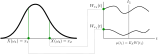
\includegraphics[width=0.8\textwidth]{./figures/randomfunction.pdf}
	\end{center}
	\caption{Example of random function $W_X$.}
	\label{fig:randomfunction}
\end{figure}

\begin{definition}[Mean of Random Function]
	Let $W$ be a continuous random function in $K$. The mean of this
	random function is
	\begin{equation}
		\mu(t) = EW(t), \ t \in K.
	\end{equation}
\end{definition}

\begin{lemma}
	If $E||W||_{\infty} < +\infty$, the $\mu$ is continuous, where
	\begin{equation}
		||W||_{\infty} := \sup_{t \in K} || W(t) ||.
	\end{equation}
\end{lemma}

These definitions are mostly used in order to rigorously define
the likelihood and the MLE, which is a point in the likelihood function,
more specifically, it's the $t^*$ that maximizes the likelihood.

\subsection{Consistency of the MLE}

\begin{theorem}[Compact MLE consistency]
	Let $W(\omega):=\log\left(\frac{f_\omega(X)}{f_\theta(X)}\right)$.
	If $\Theta$ is compact, $E_\theta ||W||_\infty < +\infty$, $f_{\omega}(x)$
	is a continuous function of $\omega$ a.e. $x$, and $P_\omega \neq P_\theta$
	for all $\omega \neq \theta$, then under $P_\theta$, $\hat \theta_n \to_p \theta$,
	where $\hat\theta_n$ is the maximum likelihood for $X_1,...,X_n$ i.i.d with
	distribution $P_\theta$.

	This theorem is implying that if the parameter space is compact and
	the likelihood functions are continuous, then the MLE is consistent.
\end{theorem}

The next theorem also shows the consistency of the MLE, but for the case
where the parameter space is not limited.

\begin{theorem}[MLE consistency]
	Let $W(\omega):=\log\left(\frac{f_\omega(X)}{f_\theta(X)}\right)$.
	If $\Theta = \mathbb R^p$, $f_\omega(x)$ is a continuous function
	of $\omega$ for a.e $x$, $P_\omega \neq P_\theta$ for all
	$\omega \neq \theta$ and $f_\omega(x) \to 0$ as $|\omega| \to +\infty$.
	If $E_\theta ||\mathbbm 1_C W||_\infty < +\infty$ for every compact
	$C \subset \mathbb R^p$, and if $E_\theta \sup_{|\omega|>a}W(\omega)<+\infty$
	for some $a>0$, then under $P_\theta$, $\hat \theta_n \to_p \theta$.
\end{theorem}

Both theorems show that the MLE is a consistent estimator, but they say nothing
about the rate of convergence. This is shown in the following theorem.

\begin{theorem}[Rate of Convergence MLE]
	Assume:
	\begin{enumerate}
		\item $X_1,X_2,...$ are i.i.d with density $p_\theta$, for $\theta \in \Theta \subset \mathbb R$;
		\item The set $A=\{x: p_\theta(x)>0\}$ is independent of $\theta$;
		\item For every $x \in A$, $\partial^2 p_\theta(x)/\partial\theta^2$ exists and is continuous in $\theta$;
		\item Let $W(\theta) = \log p_\theta(X)$. The Fisher information $I(\theta)$ for a single
		      observation exists, is finite, and $I(\theta) = E_\theta W'(\theta)^2 = -E_\theta W''(\theta)$;
		\item For every $\theta$ in the interior of $\Theta$, there exists $\varepsilon >0$ such
		      that $E_\theta || \mathbbm 1_{[\theta-\varepsilon, \theta+\varepsilon]}||_{\infty}< +\infty$;
		\item The MLE $\hat \theta_n$ is consistent.
	\end{enumerate}

	Then for any $\theta \in \Theta^\circ$,
	\begin{equation}
		\frac{\hat \theta_n - \theta}{\sqrt{n}} \rightharpoonup N\left(0,\frac{1}{I(\theta)}\right).
	\end{equation}
\end{theorem}

\subsection{Confidence Intervals}

\begin{definition}[Confidence Interval]
	If $\delta_0, \delta_1$ are statistics, then the random interval $(\delta_0,\delta_1)$
	is called a $(1-\alpha)$ confidence interval for $g(\theta)$ if
	\begin{equation}
		P_\theta(g(\theta)\in (\delta_0,\delta_1))\geq 1- \alpha,
	\end{equation}
	for all $\theta \in \Theta$. A set $S = S(X)$ is called a $1-\alpha$
	confidence region for $g(\theta)$ if
	\begin{equation}
		P_\theta(g(\theta)\in S) \geq 1-\alpha,
	\end{equation}
	for all $\theta \in \Theta$.
	Note that the confidence intervals vary with the observed data, hence,
	it is itself a random variable.
\end{definition}

\begin{definition}[Pivots]
	A variable $X$ is a pivot if the distribution of $X$ does not depend on the
	unknown parameters. They are usually useful for the construction of
	confidence intervals.
\end{definition}

\begin{example}
	Let $X_1,...X_n$ i.i.d from $N(\mu,\sigma^2)$, thus
	\begin{align*}
		Z & = \frac{\overline X_n - \mu}{\sigma/\sqrt n} \sim N(0,1) \\
		V & = \frac{(n-1)S^2}{\sigma^2} \sim \chi_{n-1}^2
	\end{align*}
	are pivots. Note that the distributions are not dependent on the parameters,
	but the functions are. Let's construct the confidence intervals
	such that $P_\theta(\mu \in (\delta_0,\delta_1)) = 1-\alpha$. To do this,
	note that $T = \frac{Z}{\sqrt(V/(n-1))}$ is pivotal also, with t-distribution
	of $n-1$ degrees of freedom.
	\begin{equation}
		(\delta_0,\delta_1):=\left(
		\overline X_n - t_{\alpha/2, n-1}\frac{S}{\sqrt n},
		\overline X_n + t_{\alpha/2, n-1}\frac{S}{\sqrt n}
		\right),
	\end{equation}
	where $t_{\alpha/2,n-1}$ is the $\alpha/2$ percentile of the t-distribution
	with $n-1$ degrees of freedom, i.e.
	\begin{equation}
		P(T \geq t_{\alpha/2,n-1}) = \int_{t_{\alpha/2,n-1}}^{\infty}
		p_{T_{n-1}}(x)d(x) = \frac{\alpha}{2}
	\end{equation}
\end{example}

\section{Hypothesis Testing}

\subsection{Likelihood ratio}
Two hypothesis $H_0$ (null hypothesis) and $H_1$ (alternative hypothesis)
consists of subsets of the parameter space $\Theta$. In other words,
if $H_0 \subset \Theta$ is the true hypothesis, it means that
$X \sim P_\theta$ such that $\theta \in H_0$, and similarly for the alternative
hypothesis. Hence, Hypothesis testing consists in defining a methodology
in order to decide which hypothesis should be ``picked''.

It's possible to reformulate this problem in our decision theory
framework. This would be equivalent to establishing a loss function
% where $L(\theta, T(X)) = \mathbbm 1_$

\subsection{Generalized Likelihood Ratio}

The Pearson-Neymman Lemma proves that the Likelihood Ratio
is the best for the case of simple hypothesis
(i.e. $H_0 = \{\theta_0\}$ and $H_1 =\{\theta_1\}$).
Yet, this test may be extended for more general hypothesis
by using the $\sup_{\theta \in H_0}$ or the MLE (when
the maximum exists). Thus, the Generalized Likelihood Ratio test
uses
\begin{equation}
	\lambda(\theta) := \frac{\sup_{\theta \in H_1} \ell(\theta)}{\sup_{\theta \in H_0} \ell(\theta)}.
	\label{eq:GenearlizedLikelihood}
\end{equation}


\section{Bootstrap}


\section{Inequalities Galore}

This section is a collection of useful inequalities related to Statistics. Here are
inequalities that are not directly related to statistics, and are more ``auxiliary'',
for example, the famous Cramér-Rao inequality is presented in Section \ref{fisher-cramer-rao}.

\begin{theorem}[Jensen's Inequality]
	Let $(\Omega, \mathcal F, P)$ be a probability space, $f:\mathbb R \to \mathbb R$
	a convex function and $X:\Omega \to \mathbb R$ a random. Then
	\begin{equation}
		f(EX) \leq E f(X).
	\end{equation}
	If $f$ is strictly convex, then the inequality is strict unless
	$X$ is almost surely constant.
\end{theorem}

\begin{theorem}[Cauchy-Schwarz]
	The famous Cauchy-Schwarz inequality has the following form
	\begin{equation}
		\left(\sum_{i=1}^n a_i b_i\right)^2 \leq \sum_{i=1}^n a_i^2 \sum_{j=1}^n b_j^2.
	\end{equation}
	We can extend this for vectors and inner products. Let $\bm u, \bm v$ be vectors
	in $\mathbb R^n$, then
	\begin{equation}
		\langle \bm u, \bm v \rangle \leq
		\sqrt{\langle \bm u, \bm u \rangle}
		\sqrt{\langle \bm v, \bm v \rangle} =
		||\bm u ||\cdot || \bm v ||
	\end{equation}.
\end{theorem}

\begin{theorem}[Covariance Inequality]
	Let $X$ and $Y$ be random variables, then
	\begin{equation}
		Cov(X,Y)^2 \leq Var(X) Var(Y).
	\end{equation}
\end{theorem}
\begin{prf}
	If the random variables have finite variance, then $E[XY]$ is an inner product,
	hence by Cauchy-Schwarz
	\begin{equation*}
		E[XY]^2 \leq E[X^2]E[Y^2]
	\end{equation*}
	Note that for $W = X - E[X]$ and $Z = Y - E[Y]$ we have
	\begin{equation*}
		E[WZ]^2 = Cov(X,Y)^2 \leq E[W^2]E[Z^2] = Var(X)Var(Y),
	\end{equation*}
	and we conclude the proof of the desired inequality.
\end{prf}

\begin{theorem}[General form of Chebyshev's Inequality]
	Let $X$ be a random variable and $g(X)>0$  be a non-decreasing
	function on $\mathbb R$. Then, for any $x$,
	\begin{equation}
		P(X \geq x) \leq \frac{E g(X)}{g(x)}.
	\end{equation}
	Note that if $Y = |X - EX|$ and $g(Y) = Y^2$, we get the standard Chebyshev's Inequality
	\begin{equation}
		P(Y \geq x)= P(|X - EX| \geq x) \leq \frac{E |X - EX|^2}{x^2}.
	\end{equation}
\end{theorem}

\section{Distributions Zoo}
This section contains a collection of important distributions and some of
their properties and derivations.

\begin{shaded}\textbf{Normal Distribution}
	For $X \sim N(\mu, \sigma^2)$ we have the density function
	\begin{equation}
		p(x) = \frac{1}{\sqrt \pi \sigma} e^{-\frac{(x-\mu)^2}{2\sigma^2}}.
	\end{equation}
	A $N(0,1)$ is called standard Normal distribution. From a
	standard Normal, if $X \sim N(0,1)$,
	for $Z = \sigma X + \mu$ then $Z \sim N(\mu,\sigma^2)$.
\end{shaded}

\begin{shaded}\textbf{$\bm{\chi^2}$ Distribution}
	The $\chi^2_k$ is the sum of the squares of $k$ independent
	random variables with standard Normal distribution.
	The density function is
	\begin{equation}
		p(x) = \frac{x^{\frac{k}{2}-1}e^{-x/2}}{2^{k/2} \Gamma(\frac{k}{2})}
		\mathbbm 1_{(0,+\infty)}(x).
	\end{equation}
\end{shaded}

\begin{shaded}\textbf{Gamma Distribution}
	The Gamma distribution is a generalization of the $\chi^2$
	distribution, i.e. a $\chi^2_1$ is a Gamma with 1 degree of freedom.
\end{shaded}

\begin{shaded}\textbf{F-Distribution}
	The F-Distribution can be obtained as the reason between
	two $\chi^2_{k_1}$ and $\chi^2_{k_2}$ random variables, i.e.
	$F(k_1, k_2) = \frac{X/k_1}{Y/k_2}$ where
	$X \sim \chi^2_{k_1}$ and
	$Y \sim \chi^2_{k_2}$.
\end{shaded}

\begin{shaded}\textbf{t-Distribution}
	\vspace{5mm}

	Let $Z \sim N(0,1)$, $V \sim \chi_{n-1}^2$, then
	\begin{equation}
		T = \frac{Z}{\sqrt{\frac{V}{n-1}}} \sim
		t_{n-1}.
	\end{equation}
	The density function for the distribution is
	\begin{equation}
		p_T(x) = \frac{\Gamma(\frac{\nu+1}{2})}{\sqrt{\nu\pi}\Gamma(\nu/2)
			(1+\frac{x^2}{\nu})^{(\nu+1)/2}},
	\end{equation}
	where $\nu = n-1$. Also, remember that
	\begin{equation}
		\Gamma(z) = \int_0^{+\infty}x^{z-1}e^{-x}dx, \ z>0.
	\end{equation}
	Which implies that $\Gamma(n) = (n-1)!$ for $n\in \mathbb N$.
\end{shaded}
